\documentclass[12pt]{article}

\usepackage{graphicx}
\usepackage[portuguese]{babel}
\usepackage[section]{placeins}
\usepackage{float}

\usepackage{listings}
\usepackage{xcolor}

\usepackage[utf8]{inputenc}

\definecolor{codegreen}{rgb}{0,0.6,0}
\definecolor{codegray}{rgb}{0.5,0.5,0.5}
\definecolor{codepurple}{rgb}{0.58,0,0.82}
\definecolor{backcolour}{rgb}{1,1,1}

\lstdefinestyle{mystyle}{
    backgroundcolor=\color{backcolour},   
    commentstyle=\color{codegreen},
    keywordstyle=\color{magenta},
    numberstyle=\tiny\color{codegray},
    stringstyle=\color{codepurple},
    basicstyle=\ttfamily\footnotesize,
    breakatwhitespace=false,         
    breaklines=true,                 
    captionpos=b,                    
    keepspaces=true,                 
    numbers=left,                    
    numbersep=5pt,                  
    showspaces=false,                
    showstringspaces=false,
    showtabs=false,                  
    tabsize=2
}

\lstset{style=mystyle}

\graphicspath{ {figures} }

\author{João Vitor Maia Neves Cordeiro (19100532) \and Bernardo Schmidt Farias (19100519)}
\title{Trabalho I - Suguru Solver em Haskell}
\date{\today}

\begin{document}

\maketitle

\section{Introdução}

Dentre os dois problemas disponíveis o grupo optou por resolver o jogo Suguru, também conhecido como Tectonic Puzzle. O jogo consiste em um puzzle semelhante ao Sudoku, porém com regras ligeiramente diferentes. Dado um tabuleiro de NxN casas, com áreas internas definidas, o jogador precisa organizar números da seguinte forma:

\begin{itemize}
    \item Uma área de tamanho M deve ser preenchida com números de 1 até M, que apareçam exatamente uma vez dentro da área.
    \item Não devem existir números iguais em casas ortogonais ou diagonais.
    \item Todo o tabuleiro deve ser preenchido.
\end{itemize}

Um exemplo de tabuleiro 8x8 e sua versão resolvida podem ser vistos abaixo:

\begin{figure}[H]
    \centering
    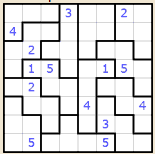
\includegraphics[width=0.25\linewidth]{example.png}
    \caption{Tabuleiro 8x8 de Suguru}
\end{figure}

\begin{figure}[H]
    \centering
    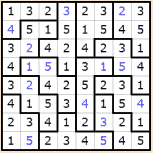
\includegraphics[width=0.25\linewidth]{solved.png}
    \caption{Tabuleiro anterior resolvido}
\end{figure}

\section{Metodologia}

Todo o trabalho foi desenvolvido em dupla, utilizando como ferramentas o Discord (para comunicação) e a extensão VSCode Live Share que permite iniciar sessões remotas colaborativas de edição de código. 

Para resolver o problema passamos por várias etapas, a primeira sendo a compreensão do puzzle e algumas "partidas" manuais dele, assim poderiamos entender melhor o funcionamento e pensar em estratégias para resolver. Depois tentamos uma primeira solução em uma linguagem de programação que o grupo possuia mais costume, a linguagem escolhida foi Python e tivemos sucesso em resolver dessa forma, o código fonte se encontra no mesmo repositório do projeto. Abaixo uma \emph{screenshot} do script Python resolvendo o exemplo dado acima em poucos milissegundos, ele utiliza \emph{backtracking} e já possui algumas otimizações.

\begin{figure}[H]
    \centering
    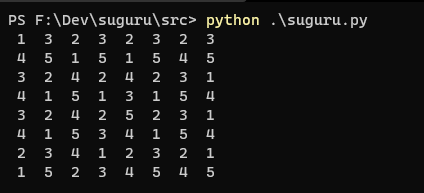
\includegraphics[width=0.75\linewidth]{python_solver.png}
    \caption{Tabuleiro anterior resolvido}
\end{figure}

Por último, com uma boa ideia de como seria o algoritmo para resolver o puzzle, partimos para a solução em Haskell que será detalhada a seguir.

\section{Solução em Haskell}

\subsection{Modelagem dos tipos}

A primeira barreira encontrada, tanto na solução em Python quanto em Haskell, foi a modelagem do tabuleiro, pois diferentemente do tabuleiro de sudoku que possui áreas fixas, o suguru pode assumir várias formas. Logo, além de receber como input o valor inicial de cada casa do tabuleiro também precisariamos de alguma forma receber o formato das áreas. 

Nas duas soluções, optamos por receber junto do valor de cada casa um identificador dizendo a qual área do tabuleiro essa casa pertence, os identificadores iriam de 0 até o número de áreas totais do tabuleiro, e a ordem escolhida como convenção foi de numerar a partir do \emph{top-left}. 

Em Haskell, criamos o tipo \texttt{Point}, como uma tupla contendo \texttt{Value} e \texttt{Sector}, e esses tipos Value e Sector são apenas \emph{aliases} para \texttt{Int}. Dessa forma, o nosso tabuleiro, nomeado como o tipo \texttt{Board} é uma matriz de \texttt{Point}. Abaixo está o código com nessas declarações de tipo exatas.

\begin{lstlisting}[language=Haskell]
-- O identificador de setor utilizado
type Sector = Int

-- Um valor de 1 a N, onde N e o tamanho do setor no qual o ponto esta
type Value = Int

-- Um par de coordenadas X, Y
type Location = (Int, Int)

-- Um ponto no tabuleiro, no formato (Value, Sector)
type Point = (Value, Sector)

-- Um tabuleiro de Suguru
type Board = [[Point]]
\end{lstlisting}

Em ambos os códigos, a entrada é dada diretamente no código por uma matriz de tuplas (Haskell) ou uma matriz de \texttt{Point} (Python). A saída do programa é mostrada no terminal após a execução. 

\subsection{Funções auxiliares}

Tendo os tipos já modelados, escrevos algumas funções auxiliares para esses tipos, por exemplo funções como \texttt{getValue} e \texttt{getSector} que recebem um ponto e retornam respectivamente seu \texttt{Value} e \texttt{Sector}. Existem outras funções como essa que servem apenas para buscar e acessar valores dentro das nossos tipos customizados, todas elas funcionam de forma parecida e trivial, portanto vamos demonstrar abaixo apenas as duas citadas acima, as outras podem ser vistas no código fonte.

\begin{lstlisting}[language=Haskell]
-- Retorna o setor de um ponto
getSector :: Point -> Sector
getSector (_, sector) = sector

-- Retorna o valor de um ponto
getValue :: Point -> Value
getValue (value, _) = value
\end{lstlisting}

Com essas funções auxiliares já podemos começar a implementar a primeira parte da nossa lógica. Dividimos a lógica basicamente em duas partes: a primeira parte checa se é possível adicionar um valor \texttt{V} em um ponto de coordenadas \texttt{(X, Y)} dentro da matriz do tabuleiro, enquanto a segunda parte utiliza \emph{backtracking} para verificar cada posição e seus pontos possíveis, gerando recursivamente o resultado final (ou retornando a matriz inicial caso não exista uma solução possível).

\subsection{Checando viabilidade do valor}

Para checarmos se um valor por ser adicionado a um determinando ponto sem quebrar as regras precisamos realizar duas verificações iniciais: verificar se no setor interno existe um outro ponto já com o mesmo valor e verificar se existem pontos vizinhos com o valor.

Para a primeira verificação, utilizamos duas funções, sendo que uma filtra a matriz do tabuleiro em busca de todos os pontos do setor \texttt{N}, enquanto a outra filtra a lista de pontos do setor \texttt{N} em busca de valores \texttt{X}, retornando \texttt{True} caso o valor exista em pelo menos um ponto.

\begin{lstlisting}[language=Haskell]
-- Retorna todos os pontos de um setor indicado pelo indice n
-- Primeiro acessando a linha, depois acessando a coluna.
getSectorPoints :: Board -> Sector -> [Point]
getSectorPoints board n = [(board !! row) !! col | row <- [0 .. size], col <- [0 .. size], getSector ((board !! row) !! col) == n]

-- Checa a existencia de um ponto com o valor [value] no [sector]
sectorHasValue :: Board -> Sector -> Value -> Bool
sectorHasValue board sector value =
    not ( null ( [point | point <- getSectorPoints board sector, getValue point == value] ) )
\end{lstlisting}

Para a segunda, utilizamos uma checagem baseada em offsets, então para um ponto na localização \texttt{(X, Y)} nós checamos os 8 pontos vizinhos baseado nas coordenadas deles, utilizando uma comparação \texttt{OR} para garantir que caso algum valor igual seja encontrado a função retorne \texttt{True}.

\begin{lstlisting}[language=Haskell]
-- Checa os valores adjacentes de determinada localizacao
-- Retorna True caso ache um ponto igual ao valor fornecido, False caso o contrario
checkAdjacents :: Board -> Location -> Value -> Bool
checkAdjacents board location v = 
  checkAdjacent board (getX location,     getY location - 1 ) v ||
  checkAdjacent board (getX location + 1, getY location - 1 ) v ||
  checkAdjacent board (getX location + 1, getY location     ) v ||
  checkAdjacent board (getX location + 1, getY location + 1 ) v ||
  checkAdjacent board (getX location,     getY location + 1 ) v ||
  checkAdjacent board (getX location - 1, getY location + 1 ) v ||
  checkAdjacent board (getX location - 1, getY location     ) v ||
  checkAdjacent board (getX location - 1, getY location - 1 ) v

-- Checa um valor adjacente
checkAdjacent :: Board -> Location -> Value -> Bool
checkAdjacent board target v
  | (getX target < 0) || (getY target < 0) = False
  | (getX target >= size) || (getY target >= size) = False
  | v == getValueFromLocation board target = True
  | otherwise = False
\end{lstlisting}

\subsection{Backtracking}

Com essas duas verificações somos capazes de saber é possível adicionar um valor a uma casa do tabuleiro sem quebrar as regras do tabuleiro já montado, mas ainda precisamos de uma maneira de iterar pelos campos e adicionar esses valores. Essa iteração não pode ser um simples loop pois um valor que inicialmente é válido pode ser mostrar um valor errado numa futura iteração, fazendo com que ele deva ser mudado. Para isso, utilizamos a técnica de \emph{backtracking} que recursivamente avança na solução, testando novos valores e desfazendo seus passos anteriores caso chegue a um "dead end".

Para isso, decidimos como convenção sempre preencher os valores na ordem \emph{top-left}, procurando o próximo campo vazio do tabuleiro, verificando um valor válido para ele e avançando. Caso após um número de iterações perceba-se que não existem mais valores possíveis a serem preenchidos a função retorna para um estado anterior do tabuleiro e tenta novamente incrementando o valor de entrada. Após testar todos os valores possíveis e não encontrar solução sabemos que o tabuleiro é insolúvel.

Quando implementamos essa solução em Python, utilizando programação imperativa, tivemos sucesso com um código relativamente simples, nossa função \texttt{solve()} possuia menos de 20 linhas e pode ser vista abaixo

\begin{lstlisting}[language=Python]
def solve(inputBoard: Board):
    row, column = nextEmpty(board)

    if row is None:
        return True

    sector_points = list(filter(lambda p: p.sector == board.points[row * board.size + column].sector, board.points))

    for i in range(1, len(sector_points) + 1):
        if check(board, row, column, i):
            board.points[row * board.size + column].value = i
        
            if(solve(board)):
                return True

        board.points[row * board.size + column].value = 0
\end{lstlisting}

Entretanto, ao tentar passar a solução para Haskell, obviamente com uma abordagem ligeiramente diferente por se tratar de uma linguagem funcional, não conseguimos uma solução correta. O maior problema encontrado durante as tentativas sempre era "desfazer" os passos realizados ao se chegar em um "dead end". Quando estavamos no Python, podiamos simplesmente alterar os pontos da variável que guardava o tabuleiro para retornar a um estado anterior. 

Em Haskell, por trabalharmos com a matriz de pontos em uma constante que era copiada a cada iteração, não poderiamos utilizar essa solução. A solução final que conseguimos em Haskell itera por boa parte da matriz, conseguindo um resultado muito próximo do correto, mas ainda assim errado. Sabemos que o erro está provavelmente na função que \texttt{solve} que implementa o \emph{backtracking}, entretanto mesmo após bastante tempo desprendido ainda não conseguimos consertar.

\section{Considerações finais}

Mesmo sabendo que o projeto ainda apresenta problemas quanto a implementação, acreditamos que a lógica utilizada esteja correta, e possivelmente com um pouco mais de familiariade com a linguagem Haskell conseguiriamos chegar numa solução satisfatória. Infelizmente o tempo de entrega (mesmo com a extensão dada pelo professor) está a poucas horas no futuro, por isso decidimos por finalizar o relatório com a solução incompleta em Haskell, explicando os problemas no caminho e demonstrando também a solução em Python.

O código, assim como os arquivos fonte desse mesmo relatório se encontram em um repositório Git, na url \texttt{https://github.com/Leviosar/suguru}.

\medskip

\end{document}